\documentclass[11pt]{beamer}
\usetheme{Montpellier}
\usecolortheme{orchid}
\usepackage[utf8]{inputenc}
\usepackage[german]{babel}
\usepackage[T1]{fontenc}
\usepackage{amsmath}
\usepackage{amsfonts}
\usepackage{amssymb}
\usepackage{graphicx}
\usepackage{url}
\usepackage[export]{adjustbox}

\usepackage{tikz}
\usetikzlibrary{positioning, arrows}
\tikzset{
block/.style={
  draw, 
  rectangle, 
  minimum height=1.5cm, 
  minimum width=3cm, align=center
  }, 
line/.style={->,>=latex'}
}
\def\checkmark{\tikz\fill[fill=green!50!black,scale=0.4](0,.35) -- (.25,0) -- (1,.75) -- (.25,.15) -- cycle;} 

\author{Patrick M\"unnich}
\title{Identifizierung des Sigmatismus Lateralis in Audioaufnahmen}
%\setbeamercovered{transparent}
\setbeamertemplate{navigation symbols}{} 
\institute{Hochschule D\"usseldorf} 
%\date{} 
\subject{Signalverarbeitung} 
\begin{document}

%\begin{frame}
%\titlepage
%\end{frame}

\section{Inhaltsverzeichnis}

\begin{frame}
\tableofcontents
\end{frame}

\section{Sigmatismus Lateralis}

\begin{frame}
\frametitle{Sigmatismus Lateralis}
\begin{figure}
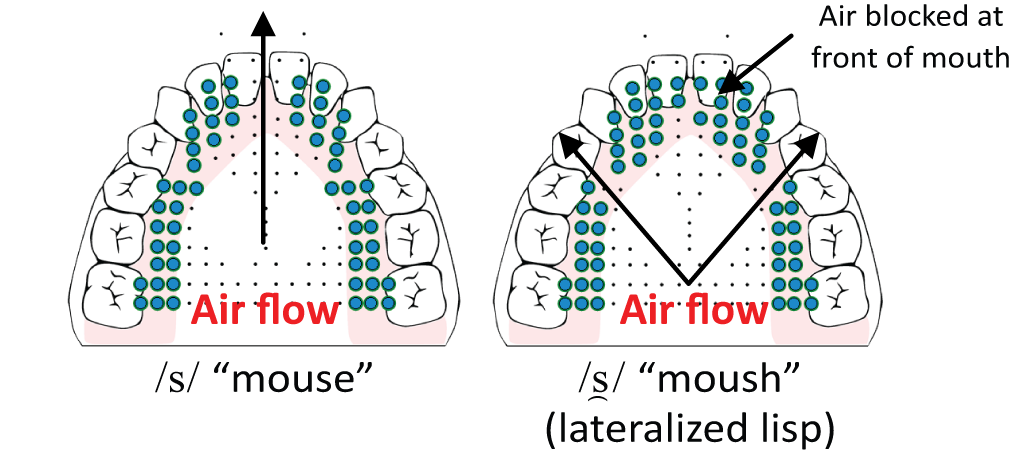
\includegraphics[scale=0.4]{lateral_lisp.png}
\caption{Sigmatismus Lateralis (SL) verglichen mit normalem ''s''. (\url{https://www.pinterest.com/pin/7248049373293660/})}
\end{figure}
\end{frame}

\begin{frame}
\frametitle{Sigmatismus Lateralis Video}
\centering
\url{https://youtu.be/Y3mEaV1kCiU?t=21}
\end{frame}

\section{Vergleich von FFTs}

\subsection{Vergleichsparameter}

\begin{frame}
\frametitle{Vergleichsparameter}
\begin{itemize}
\item Einfache Aufnahme mit Clip-on Mikrofon neben Mund
\item 16-bit mono mit $f_\mathrm{sampling}=8000$\,Hz
\item Insgesamt drei Aufnahmen
\item Alle Aufnahmen nur stimmloses ''s'' Ger"ausch mit oder ohne Lispeln
\end{itemize}
\end{frame}

\subsection{Vergleich}

\begin{frame}
\frametitle{Vergleich von FFTs}
\begin{figure}
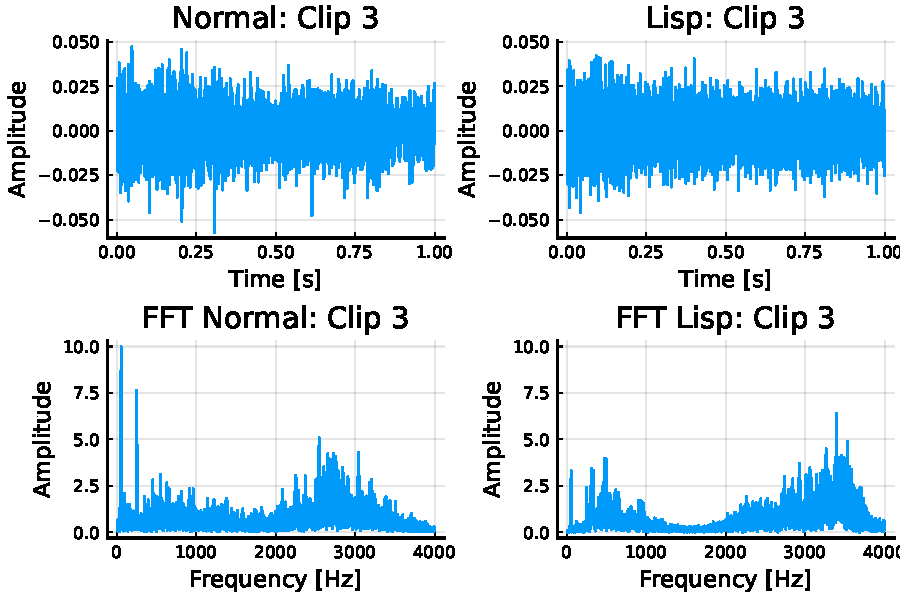
\includegraphics[scale=0.5]{../output/normal_vs_lisp_clip_3.pdf}
\caption{Beispielsweiser Vergleich der FFTs vom normalen ''s'' und SL.}
\end{figure}
\end{frame}

\subsection{Analyse}

\begin{frame}
\frametitle{Feststellungen bei Vergleich von FFTs}
\begin{itemize}
\item[$\Rightarrow$] Bei allen drei Aufnahmen offensichtlich viel mehr im h"oheren Frequenzbereich (ca.\ 1200-3500\,Hz)
\item[$\Rightarrow$] Ansatz: man sollte durch Vergleich der h"oheren Frequenzen zwischen normalen ''s'' und SL unterscheiden k"onnen
\end{itemize}
\end{frame}

\begin{frame}
\frametitle{Codediagramm}
\begin{figure}
\scalebox{0.5}{
\begin{tikzpicture}

\node[block]	(read)														{Audiodatei \\ einlesen};
\node[block]	(parameters)		[above right=0.2cm and 2cm of read]			{Parameter \\ feststellen};
\node[block]	(subtraction)	[below right=0.2cm and 2cm of read]			{Subtraktion des \\ Mittelwerts};
\node[block]	(normalizesub)	[right=of subtraction]						{Normalisierung};
\node[block]	(absfft)			[right=of normalizesub]						{Absolutwerte \\ FFT};
\node[block]	(slice)			[below right=1cm and 2cm of absfft]			{Begrenzung auf \\ bestimmte Frequenzen};
\node[block]	(plot)			[above=4.5cm of slice]					{Plotten};
\node[block]	(normalizefft)	[left=of slice]								{Normalisierung};
\node[block]	(mean)			[left=of normalizefft]						{Mittelwerte \\ berechnen};
\node[block]	(findmax)		[left=of mean]								{Maximalwert \\ finden};
\node[block]	(thresh)			[left=of findmax]							{Verifizierung durch \\ Referenzwerte};

\draw[line] (read.north) |- (parameters.west);
\draw[line] (read.south) |- (subtraction.west);
\draw[line] (subtraction.east) -- (normalizesub.west);
\draw[line] (normalizesub.east) -- (absfft.west);
\draw[line] (absfft.east) -| (plot.south);
\draw[line] (absfft.east) -| (slice.north);
\draw[line] (parameters.east) -- (plot.west);
\draw[line] (slice.west) -- (normalizefft.east);
\draw[line] (normalizefft.west) -- (mean.east);
\draw[line] (mean.west) -- (findmax.east);
\draw[line] (findmax.west) -- (thresh.east);
\end{tikzpicture}
}
\caption{Funktionsweise des derzeitigen Codes zur Identifizierung des SL in Aufnahmen durch Vergleich der Aufnahmen}
\end{figure}
\end{frame}

\begin{frame}
\frametitle{Ergebnisse}
\begin{exampleblock}{Einfache Parameter}
Bei den derzeitigen einfachen Parametern kann der Code zwischen den beiden ''s'' Ger"auschen differenzieren und den SL sowohl identifizieren als auch verifizieren.
\end{exampleblock}

\begin{block}{Implementierung in Julia}
\url{https://github.com/munnich/lateral-lisp}
\end{block}
\end{frame}

\subsection{Einf\"uhrung anderer Parameter}

\begin{frame}
\frametitle{Vergleich mit \textit{AT2020USB+} Mikrophon}
\begin{minipage}{.5\textwidth}
\begin{figure}
\adjincludegraphics[scale=0.5, trim={{.52\width} 0 0 0}, clip]{../output/normal_vs_lisp_at_1.pdf}
\caption{Beispielsweiser Vergleich mit \textit{AT2020USB+}.}
\end{figure}
\end{minipage}
\begin{minipage}{.4\textwidth}
\begin{itemize}
\item Bereich bei SL st"arker ausgepr"agt
\item Identifizierung erfolgreich
\item Verifizierung scheitert
\end{itemize}
\end{minipage}
\end{frame}

\section{Plan}

\begin{frame}
	\frametitle{Plan}
	\begin{enumerate}
		\item Identifizierung des korrekten ''s'' durch Vergleich der Durchschnittsamplitude im Bereich 1200-3500\,Hz \checkmark
		\item Einf"uhrung verschiedener Parameter, z.B.\ Mikrofon, Position, Maske etc.\ und "Uberpr"ufung der bisherigen Methode \checkmark
		\item Methode des Skripts von Prof.\ Dederichs ausprobieren
		\item Identifizierung (in)korrekten ''s'' ohne Referenz-''s'', z.B.\ durch einfache Analyse der Durchschnittsamplitude im Frequenzbereich
		\item Idealerweise: Identifizierung eines ''s'' in einem Wort, Fenster finden und entwickeltes Verfahren anwenden 
	\end{enumerate}
\end{frame}

\section{Formanten}

\begin{frame}
\frametitle{Betrachtung der Formanten mit Praat}
Screenshots w"aren hier leider zu gro"s
\begin{block}{Ergebnisse}
\begin{enumerate}
\item Formant normal zwischen 700-800, Lispeln 500-700
\item Formant normal zwischen 1500-2000, Lispeln 1800-2200
\item[$\Rightarrow$] Schien konsistent "uber alle Aufnahmen
\end{enumerate}
\end{block}
\end{frame}

\end{document}